%\documentclass{article}
%\usepackage{graphicx,subfigure}
%\begin{document}

\begin{figure}[h]
  \centering
  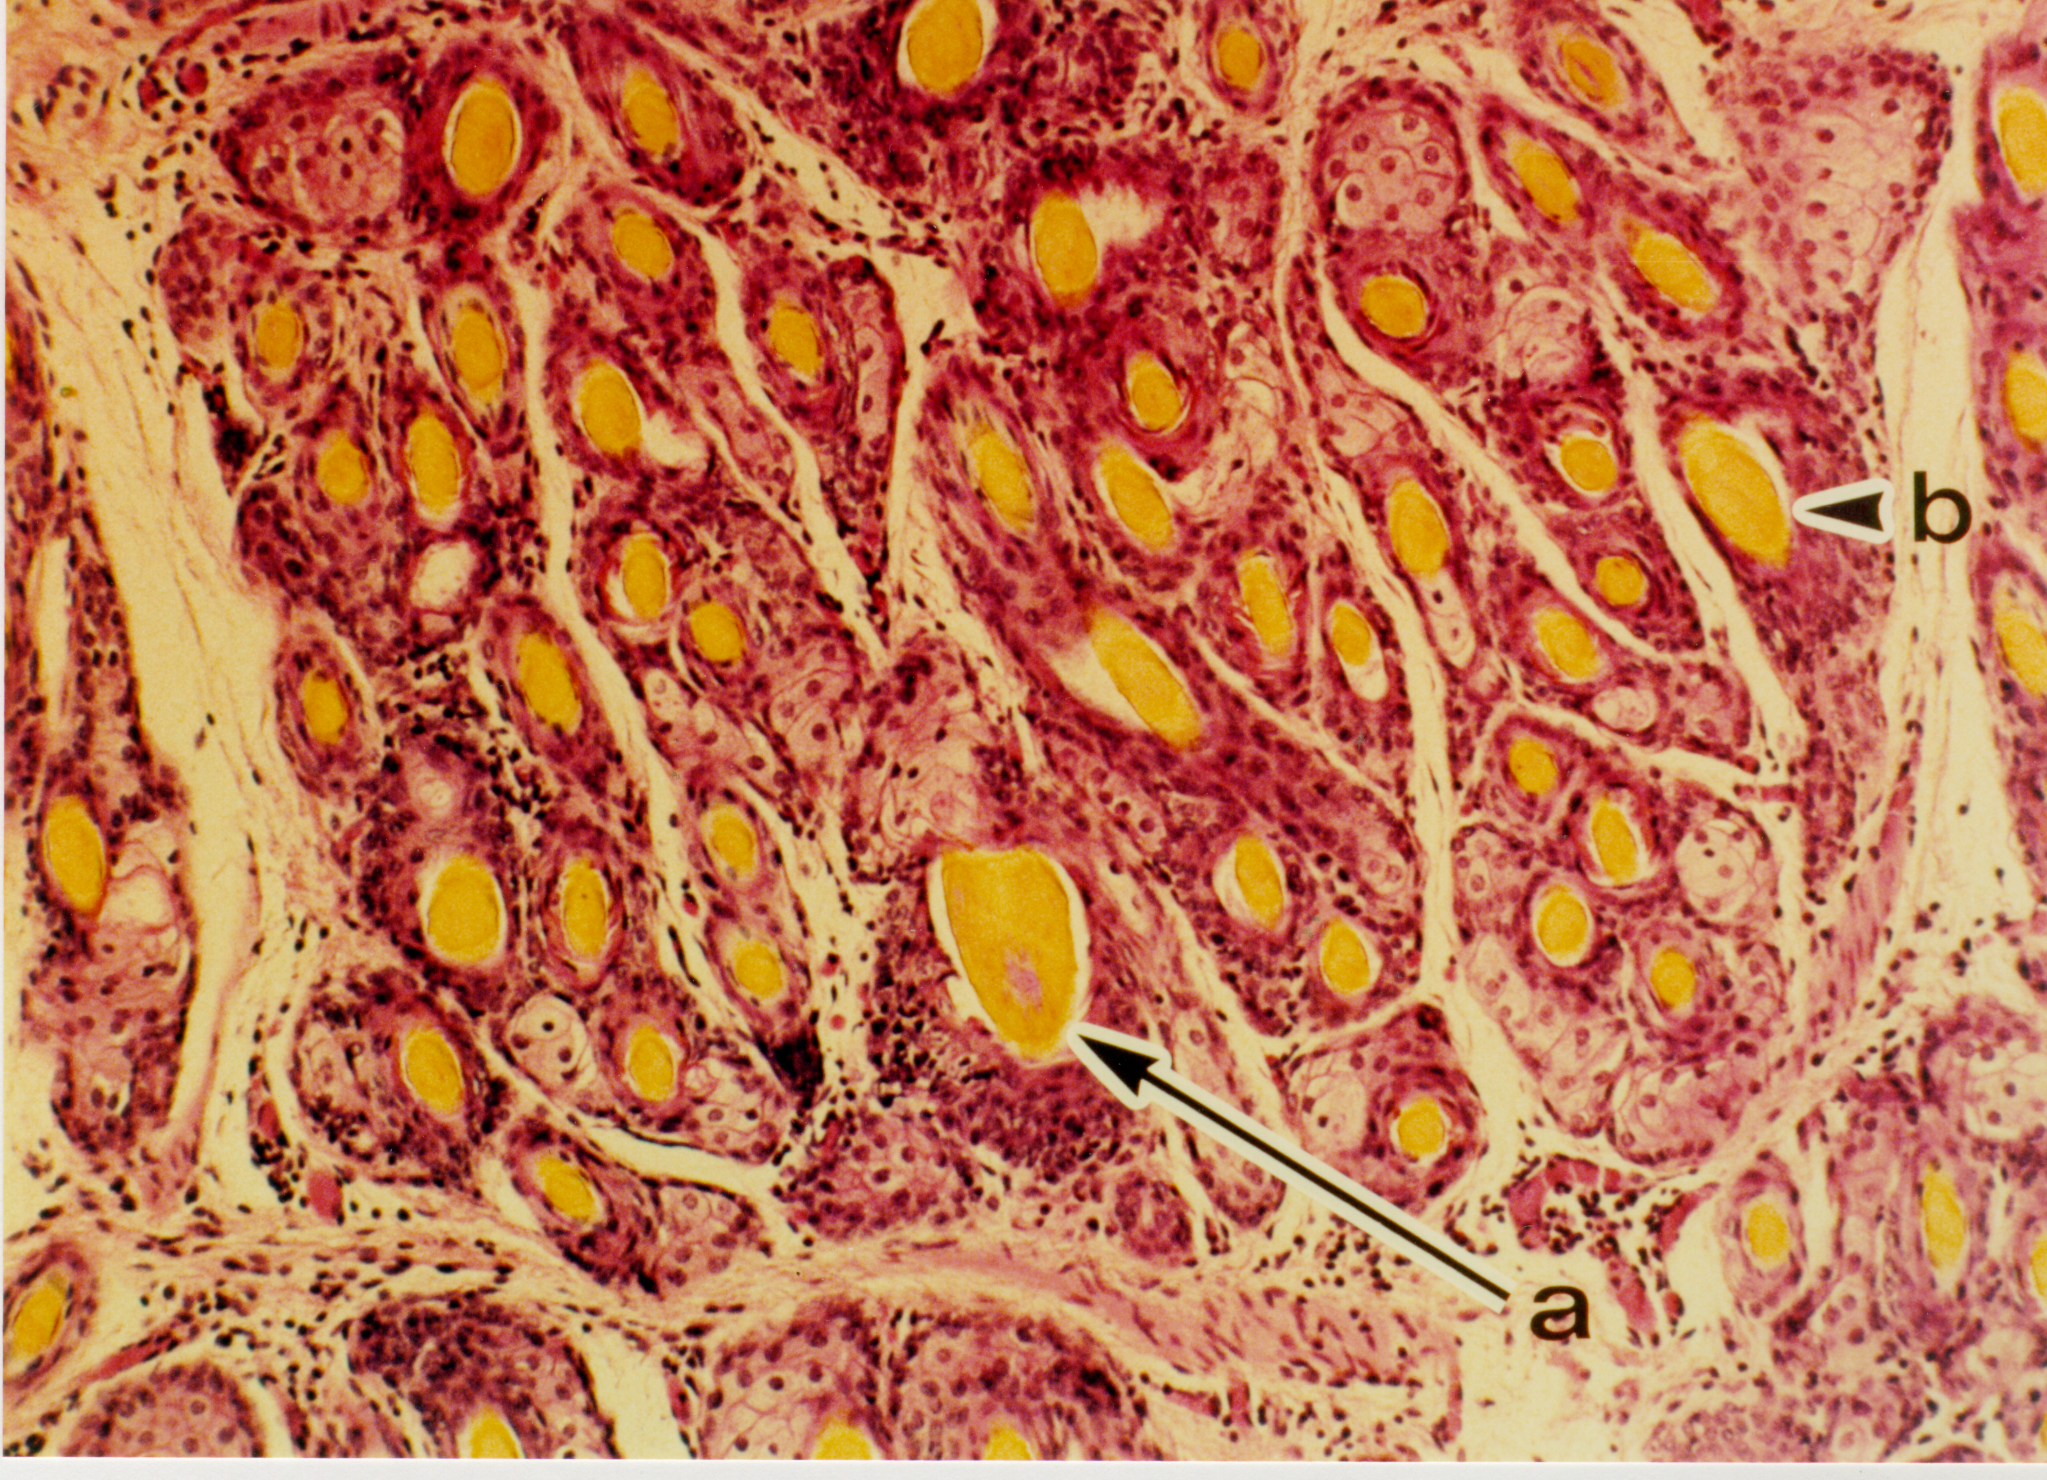
\includegraphics[width=\textwidth, trim = 0 0 0 20]{images/fig11.png}
  \caption{Transverse section of skin from the specimen of 
      Figure~\ref{fig:10}.  Note
      (a) large medullated central primary fibre and (b) large non-
      medullated lateral primary fibre.
      Plate (i) x... magnification.}
  \label{fig:11}
\end{figure}

%\end{document}
